%!TEX program = lualatex
\documentclass[14pt]{constructor-thesis}

\usepackage[backend=bibtex]{biblatex}
\usepackage{tikz}
\usepackage{import}
\addbibresource{thesis.bib}

\begin{document}
% Год, город, название университета и факультета предопределены,
% но можно и поменять.
% Если англоязычная титульная страница не нужна, то ее можно просто удалить.
\filltitle{en}{
  chair              = {Bachelor of Science \\ Computer Science},
  title              = {Mechanizing semantics of graph query languages in Coq},
  author             = {Semen Panenkov},
  supervisorPosition = {professor},
  supervisor         = {Anton Podkopaev},
  reviewerPosition   = {},
  reviewer           = {},
  chairHeadPosition  = {professor},
  chairHead          = {Christobal Junta},
}
\maketitle
\tableofcontents
% У введения нет номера главы
\section*{Introduction}

Databases have come a long way since their inception, and today we have a plethora of database types available, each designed to serve a particular use-case~\cite{database-types}. One of the more recent types to gain popularity are graph databases.

As the name suggests, graph databases represent data using graphs. While the idea of representing data with graphs isn't new with solutions developed as early as the mid-1960s, the first enterprise-ready ACID-compliant transactional database only emerged in 2007 with the release of Neo4j~\cite{enwiki:1146498781}.

Since then, many graph databases have emerged (Amazone Neptune, RedisGraph, NebulaGraph and others)~\cite{enwiki:1146498781}. They have been successfully applied in various fields such as recommendation services, fraud detection in finance~\cite{neo4j:use-cases} and even investigations of corruption schemes~\cite{icij:offshoreleaks}.

\subsection*{Property Graphs}

These databases use so-called property graphs as an underlying data model.
A property graph is a directed multigraph where each node or edge could
store a set of property-value pairs. In addition, labels can be added to nodes and edges to indicate their meaning.

\begin{figure}[b]
  \centering
  
  \import{img/}{property-graph.tex}

  % 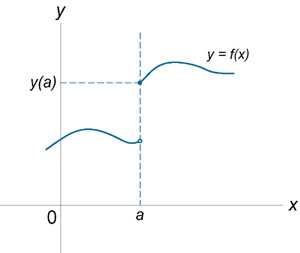
\includegraphics{img/fig1.jpg}
  \caption{Example property graph}
  \label{fig:property-graph}
\end{figure}

For instance, on figure~\ref{fig:property-graph} there are two nodes with labels ``Person'' and ``Company'', respectively. The company has a property ``name'' with a value of ``JetBrains'', and there is an edge from the person to the company labeled ``WORKS\_FOR''. As you can see, this edge also has a property.

\section{Chapter A}
Nulla malesuada porttitor diam. Donec felis erat, congue non, volutpat at, tincidunt tristique, libero. Vivamus viverra fermentum felis. Donec nonummy pellentesque ante. Phasellus adipiscing semper elit. Proin fermentum massa ac quam. Sed diam turpis, molestie vitae, placerat a, molestie nec, leo.
Maecenas lacinia~\cite{test}.







h



$\Phi$ Nam ipsum ligula, eleifend at, accumsan nec, suscipit a, ipsum. Morbi blandit ligula feugiat f magna. Nunc eleifend consequat lorem. Sed lacinia nulla vitae enim. Pellentesque tincidunt purus vel magna. Integer non enim. Praesent euismod nunc eu purus. Donec bibendum quam in tellus. Nullam cursus pulvinar lectus. Donec et mi. Nam vulputate metus eu enim. Vestibulum pellentesque felis eu massa. Quisque ullamcorper placerat ipsum. Cras nibh. Morbi vel justo vitae lacus tincidunt ultrices. Lorem ipsum dolor sit amet, consectetuer adipiscing elit. In hac habitasse platea dictumst. Integer tempus convallis augue. Etiam facilisis. Nunc elementum fermentum wisi. Aenean placerat. Ut imperdiet, enim sed gravida sollicitudin, felis odio placerat quam, ac pulvinar elit purus eget enim. Nunc vitae tortor. Proin tempus nibh sit amet nisl. Vivamus quis tortor vitae risus porta vehicula.

% % Рисунок, размещенный с предпочтением "вверху страницы"
% \begin{figure}[t]
% \label{discontinuities}
% \centering
% 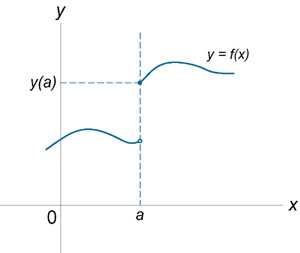
\includegraphics{img/fig1.jpg}
% \caption{Discontinuity}
% \end{figure}

% У заключения нет номера главы
\section*{Conclusion}
\lipsum[1-2]

\setmonofont[Mapping=tex-text]{CMU Typewriter Text}
% \bibliographystyle{plain}
% \bibliography{thesis}
\printbibliography
\end{document}
